\chapter{Background\label{background}}
Node.js is a asynchronous event-driven JavaScript runtime environment that is designed to build scalable network applications (\cite{node.jsAbout}).
In its core process it uses event loop at runtime to handle callbacks.
Node.js is able to perform blocking I/O event within a single runtime thread by offloading operations to system kernel when possible (\cite{node.jsEventLoop}).
These operations are called non-blocking operations or asynchronous operations (\cite{node.jsOverviewBlockVsNonBlock}).
Events that block the event loop from continuing its process are called blocking operations or synchronous operations.
Node.js itself is able to perform one event at any given time and offloading processes to kernel.

Node.js event loop consist of six phases shown in figure \ref{figure:nodejs:eventloop} (\cite{node.jsEventLoop}).
\begin{itemize}
    \item
    timers: executes callbacks scheduled by \textit{setTimeout} and \textit{setInterval} callbacks. These callbacks schedules callbacks to be called later on.
    \item
    pending callbacks: executes I/O callbacks deferred to the next loop iteration.
    \item
    idle, prepare: only used internally
    \item
    poll: retrieve new I/O events, execute I/O related callbacks.
    \item
    check: \textit{setImmediate} callbacks are invoked here. \textit{setImmediate} executes its callback in the next iteration.
    \item
    close callbacks: emits the 'close' event when socket or handler is closed abruptly
\end{itemize}

\begin{figure}[ht!]
    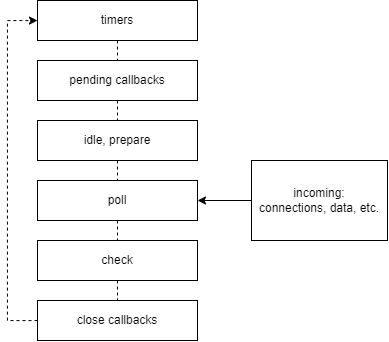
\includegraphics[scale=0.8]{images/event_loop.png}
    \caption{Simplified event loop with it phases. \cite{node.jsEventLoop}.}
    \label{figure:nodejs:eventloop}
\end{figure}

Each phase consist of first in, first out queue of callbacks waiting to be executed.
When event loop enters specific phase it performs callbacks from the queue until the queue is empty of the maximum number of events has been executed.
After that it enters the next phase continuing the process.
Any of these operations may schedule more operations.

When no timers are scheduled the poll phase executes its callbacks synchronously until its queue is empty or system limit is reached.
If there are scripts called by \textit{setImmediate}, once the poll queue is empty the event loop ends poll phase and enters the check phase.
Otherwise the event loop will wait for callbacks to be added to poll queue and execute them immediately.
Once the poll queue is empty the event loop will check for timers whose time threshold has been reached and wrap back to the timers phase.
